\documentclass[conference]{IEEEtran}
\IEEEoverridecommandlockouts

% The preceding line is only needed to identify funding in the first footnote. If that is unneeded, please comment it out.
\usepackage{cite}
\usepackage{amsmath,amssymb,amsfonts}
\usepackage{algorithmic}
\usepackage{graphicx}
\usepackage{textcomp}
\usepackage{hhline}
\usepackage{xcolor}
\usepackage{pgffor}
\usepackage{hyperref}
\usepackage{lipsum}
\usepackage{listings}
\usepackage{pifont}
\usepackage{xkvltxp}
\usepackage{fixme}
\usepackage{makecell}

\newcommand{\cmark}{\ding{51}}%
\newcommand{\xmark}{\ding{55}}%

\def\BibTeX{{\rm B\kern-.05em{\sc i\kern-.025em b}\kern-.08em
    T\kern-.1667em\lower.7ex\hbox{E}\kern-.125emX}}


\lstset{
  frame=single,
  language=clean,
  basicstyle=\small,
  captionpos=b,
  linewidth=\linewidth
}

\makeatletter
\def\lst@makecaption{%
  \def\@captype{figure}%
  \@makecaption
}
\makeatother

\newcommand{\inlinelst}[1]{\lstinline[columns=fixed]{#1}}

\fxsetup{status=draft,layout=inline,theme=color,author=}
    
%%%%%%%%%%%%%%%%%%
% Begin Document
%%%%%%%%%%%%%%%%%%
\begin{document}

\title{Evaluation of the YANG-based network management framework Clixon}

%%%%%%%%%%%%%%%%%%
% Authors
%%%%%%%%%%%%%%%%%%

\author{
    \IEEEauthorblockN{Simon Bauer}
    \IEEEauthorblockA{
        \textit{Esslingen University of} \\
        \textit{Applied Sciences} \\
        bauer-s-public@outlook.com
    }
\and
    \IEEEauthorblockN{Martin Mager}
    \IEEEauthorblockA{
        \textit{Esslingen University of} \\
        \textit{Applied Sciences} \\
        magerm.dev@gmail.com
}
\and
    \IEEEauthorblockN{Michael Scharf}
    \IEEEauthorblockA{
        \textit{Esslingen University of} \\
        \textit{Applied Sciences} \\
        michael.scharf@hs-esslingen.de
    }
}

%%%%%%%%%%%%%%%%%%
% Title
%%%%%%%%%%%%%%%%%%
\maketitle

%%%%%%%%%%%%%%%%%%
% Abstract + Keywords
%%%%%%%%%%%%%%%%%%
\begin{abstract}

YANG-based network management is gaining importance and requires corresponding implementations. This paper evaluates and compares the open source framework \textit{Clixon} with other well-known open source solutions as well as commercial alternatives. We analyze the the \textit{Clixon} framework with a prototype. As use case it implements the draft of a standard YANG model for the Transmission Control Protocol (TCP). Our results confirm that \textit{Clixon} is a a portable and extensible implementation well-suited for YANG-based management.

\end{abstract}

\begin{IEEEkeywords}
Clixon, YANG, NETCONF, network management.
\end{IEEEkeywords}

%%%%%%%%%%%%%%%%%%
% Contents
%%%%%%%%%%%%%%%%%%

\section{Introduction}
\label{sec:introduction}

State-of-the-art network management requires standardized network management protocols and data modeling languages. The Network Configuration Protocol (NETCONF)~\cite{RFC6241} and the data modeling language YANG~\cite {RFC7950} have gained acceptance among vendors of network equipment. Also other industries show interest in these standardized and field-proven technologies to handle management of complex systems. This may extend the usage of NETCONF/YANG from network devices to a wide range of industries.

The growing acceptance and usage of NETCONF/YANG drives the need for common, well-tested and future-proof management frameworks that work across many environments. While there are several commercial options available, like \textit{ConfD} from Cisco~\cite{confd}, they are mostly closed-source and do not allow for any modifications or adjustments to the base product. Besides commercial options, multiple open-source management frameworks exist, allowing companies to gain full control and adjust the framework to their individual needs.

This paper introduces and evaluates the open source network management framework \textit{Clixon} and presents a comparison of its capabilities with the well-known open source framework \textit{Netopeer2}~\cite{netopeer2} and the commercial, closed-source alternative \textit{ConfD}. \textit{Clixon} is intended for network devices and other computer systems and provides support for a large feature set, such as datastores and appropriate transaction mechanisms. Developers can easily integrate in the framework by providing plugins to react to configuration changes or return state data. To interact with the management agent, the network management protocols NETCONF and RESTCONF as well as a rudimentary command line interface (CLI) are provided~\cite{clixon-documentation}.

The rest of this paper is organized as follows. Section~\ref{sec:clixon-framework} introduces \textit{Clixon}, presents an overview of the architecture and draws a comparison with other open-source frameworks. The \textit{ietf-tcpm-yang-tcp}~\cite{draft-ietf-tcpm-yang-tcp} YANG model is introduced in Section~\ref{sec:prototype} and the corresponding \textit{Clixon} plugin is shown. In addition, the portability of the prototype and the underlying framework is analyzed. The related work is summarized in Section~\ref{sec:related-work}. Finally, Section~\ref{sec:conclusion} concludes the paper.
\section{Clixon Framework}
\label{sec:clixon-framework}

\textit{Clixon} is an open-source YANG-based configuration manager that has been developed by Olof Hagsand since 2009. 

The framework is characterized by its modular structure and plugin architecture which allows for easy extension and modification. \textit{Clixon} provides inbuilt support for datastore management and multiple common interfaces, namely \textit{CLI}, \textit{NETCONF} and \textit{RESTCONF}. 

\textit{Clixon} is targeted towards GNU/Linux and virtualized environments, like Docker, but a community driven FreeBSD port is available in addition to that. Due to the broad platform support, the framework can be used in a variety of environments and for different scenarios.

This section is structured as follows. First, the overall architecture of the framework is presented. Then, the important plugin architecture is discussed in more detail. Finally, the available features of \textit{Clixon} are compared with \textit{Netopeer2} and \textit{ConfD}.

%%%%%%%%%%%%%%%%%%
% Overall Architecture
%%%%%%%%%%%%%%%%%%
\subsection{Overall Architecture}

\textit{Clixon} is built in a modular fashion to allow for easy extension and integration. The overall system architecture is shown in Fig.~\ref{fig:architecture}, highlighting the major components of a common usage scenario~\cite{clixon-documentation, clixon-repo}.

\begin{figure}[htbp]
    \centering
    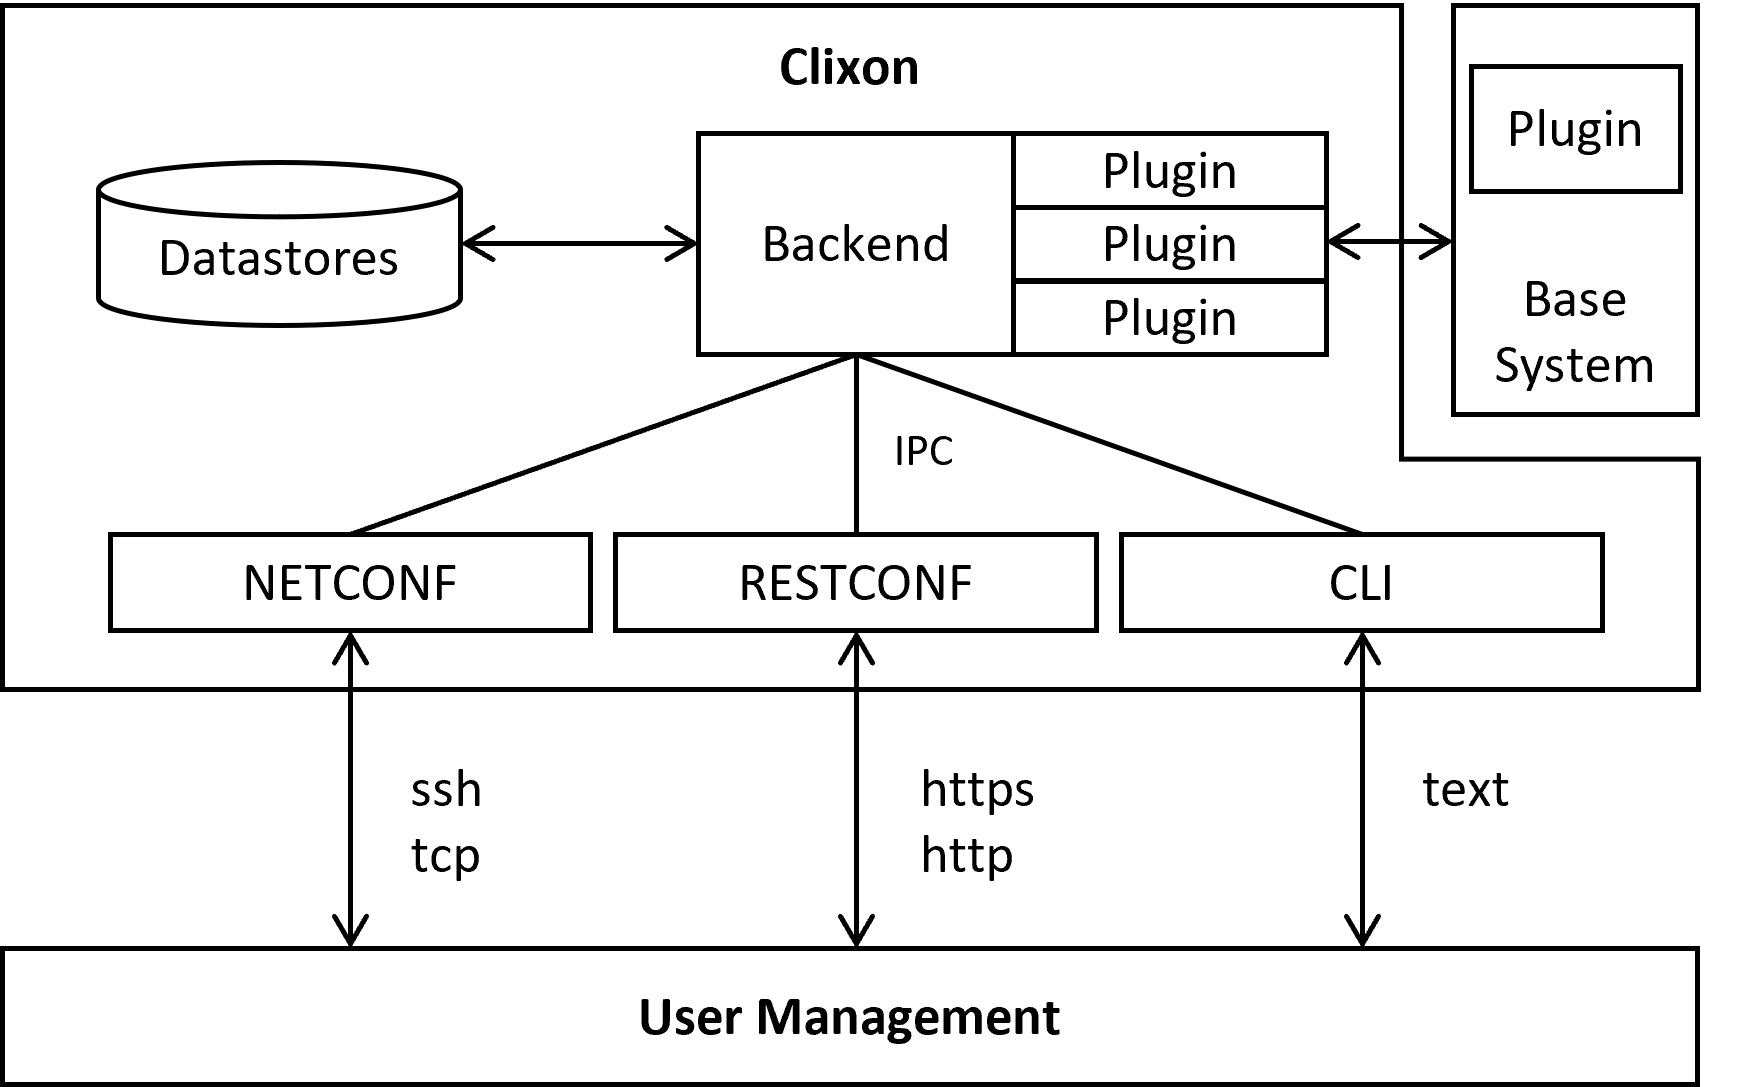
\includegraphics[width=\linewidth]{assets/3_ClixonFramework/Clixon_Architecture_v.png}
    \caption{Clixon Architecture.}
    \label{fig:architecture}
\end{figure}

\begin{enumerate}
    \item \textit{Backend}: The backend daemon handles various core functionalities of the framework. These includes tasks such as managing data stores, privileges and the plugin system. In addition, it provides a \mbox{NETCONF-based} inter-process communication (IPC) bus to enable communication with the other framework components.
    
    \item \textit{Interfaces}: The already built-in internal clients CLI, RESTCONF and NETCONF provide external interfaces for management. These includes RESTCONF over HTTP/HTTPS, NETCONF over TCP or SSH and an interactive CLI Interface. By default, the internal clients are running as separate processes that communicate with the backend via IPC.

    \item \textit{Plugins}: Plugins are shared libraries which provide the required system interaction with the base system for the various YANG specifications. Plugins attach to certain events and therefore get notified of configuration changes and are able to provide state data from the system. The Plugin architecture is discussed in more detail in section \ref{sec:clixon-framework_plugin-architecture}.

    \item \textit{Datastores}: \textit{Clixon} implements the \textit{candidate}, \textit{running}, and \textit{startup} datastores, specified in RFC 6241~\cite{RFC6241}. In addition, \textit{Clixon} provides an interface for interacting with the datastores provided, facilitating transactional workflows. Currently, \textit{Clixon} does not offer support for the Network Management Datastore Architecture (NMDA)~\cite{RFC8342} and therefore does not provide an \textit{intended} and \textit{operational} datastore. However, due to the extensible structure of the \textit{Clixon} framework, this feature can be implemented with reasonable effort.
\end{enumerate}


%%%%%%%%%%%%%%%%%%
% Plugin Architecture
%%%%%%%%%%%%%%%%%%
\subsection{Plugin Architecture}
\label{sec:clixon-framework_plugin-architecture}

The \textit{Clixon} daemon loads the YANG modules and therefore knows about the structure of the involved data. This allows \textit{Clixon} to maintain the datastores, handle read and update requests, and expose this functionality via its interfaces. The daemon on its own, however, does not have any knowledge about the semantics of the involved YANG model and in consequence is unable to apply any changes to the base system.

The semantics is provided to \textit{Clixon} in the form of plugins which implement the required logic to interact with the system. Plugins are dynamically loaded shared objects which expose a function named \inlinelst{clixon\_plugin\_init}. This method is called during startup and allows plugins to attach various callbacks to the \textit{Clixon} daemon. Besides several lifecycle events, like \inlinelst{start}, \inlinelst{daemon} and \inlinelst{exit}, the main callbacks consist of several transaction hooks, such as \inlinelst{trans\_begin}, \inlinelst{trans\_commit} and \inlinelst{trans\_abort}, and a callback to provide state data. Other useful events exist to handle YANG extension data, datastore upgrades, remote procedure call (RPC) events and system resets.

\textit{Clixon} follows NETCONF in terms of validate and commit semantics and provides the necessary infrastructure for transaction processing. Plugins usually subscribe to multiple lifecycle events of the transaction and thereby supply the logic to validate the configuration changes and incrementally upgrade the system state based on the configuration changes. \text{Clixon} provides a feature-rich XML and transaction interface that allows plugins to easily detect changes in the XML tree and act accordingly.


%%%%%%%%%%%%%%%%%%
% Feature Comparison
%%%%%%%%%%%%%%%%%%
\subsection{Feature Comparison}

There are several NETCONF/YANG frameworks with varying functionality and support for the respective standards. This section is used to compare \textit{Clixon} with two well-known alternatives, namely the open-source tool \textit{Netopeer2} and the commercial, and therefore closed-source framework \textit{ConfD}. As criteria for the comparison, the supported RFC standards are analyzed, as well as the support for XML and XPath.

\textit{Netopeer2} is a NETCONF server implementation based on the open-source projects \textit{libyang}, \textit{libnetconf2} and \textit{sysrepo}. It is in its second generation and is already well-established in the field of network management~\cite{netopeer2}.

\textit{ConfD}, developed by the \textit{Cisco} company \textit{Tail-F}, is a commercially distributed NETCONF/YANG toolset. It is available in a free and limited \textit{Basic} or paid \textit{Premium} edition. \textit{ConfD} is built on a more than 10-year development foundation and offers a variety of features that the open-source solutions cannot provide. In the following, only the premium version of \textit{ConfD} is considered~\cite{confd}.

Table~\ref{tab:clixon-features} presents a brief overview and comparison of the features provided by the above-mentioned NETCONF/YANG frameworks.

% summary

The comparison has shown that \textit{Netopeer2} is the only network management framework in the comparison that does not offer a RESTCONF interface. 
Furthermore, it is noticeable that \textit{Clixon} offers only partial support for certain standards, which in many cases is due to diverging default values or left-out features. In addition, \textit{Clixon} does not currently support NMDA for NETCONF. The commercial solution \textit{ConfD} scores best across all analyzed criteria, but comes at an expensive price.

\begin{table*}[ht]
    \caption{Feature Comparison}

    \begin{center}
        \begin{tabular}{|l|c|c|c|c|}

            % YANG
            \hline
            \textbf{YANG} &\textbf{RFC} & \textbf{\textit{Clixon}} \textit{(v5.4.0)} & \textbf{\textit{Netopeer2}} \textit{(v2.0.35)} & \textbf{\textit{ConfD}} \textit{(v7.6)} \\ 
        
            \hhline{|=|=|=|=|=|}
            YANG 1.0 & \href{https://datatracker.ietf.org/doc/html/rfc6020}{6020} & \cmark & \cmark & \cmark \\                  
            
            \hline
            YANG 1.1 & \href{https://datatracker.ietf.org/doc/html/rfc7950}{7950} & (\cmark)                 & \cmark & \cmark \\  
            
            \hline
            YANG Library & \href{https://datatracker.ietf.org/doc/html/rfc8525}{8525} & (\cmark) & \cmark & \cmark \\ 
            
            \hline
            \multicolumn{5}{c}{}\\
            
            % 
            \hline
            \textbf{NETCONF} &\textbf{RFC} & \textbf{\textit{Clixon}} \textit{(v5.4.0)} & \textbf{\textit{Netopeer2}} \textit{(v2.0.35)} & \textbf{\textit{ConfD}} \textit{(v7.6)} \\ 
            
            \hhline{|=|=|=|=|=|}
            NETCONF Event Notifications & \href{https://datatracker.ietf.org/doc/html/rfc5277}{5277} & (\cmark) & \cmark & \cmark \\ 
            
            \hline
            Network Configuration Protocol (NETCONF) & \href{https://datatracker.ietf.org/doc/html/rfc6241}{6241} & (\cmark) & \cmark & \cmark \\ 
            
            \hline
            Using the NETCONF Protocol over Secure Shell (SSH) & \href{https://datatracker.ietf.org/doc/html/rfc6242}{6242} & \cmark & \cmark & \cmark \\ 
            
            \hline
            NETCONF Call Home and RESTCONF Call Home & \href{https://datatracker.ietf.org/doc/html/rfc8071}{8071} & (\cmark) & \cmark & \cmark \\ 
            
            \hline
            Network Configuration Access Control Model & \href{https://datatracker.ietf.org/doc/html/rfc8341}{8341} & \cmark & \cmark & \cmark \\ 
            
            \hline
            NETCONF Extensions to Support the NMDA & \href{https://datatracker.ietf.org/doc/html/rfc8526}{8526} & \xmark & \cmark & \cmark \\ 

            \hline

            \multicolumn{5}{c}{}\\
            
            % RESTCONF
            \hline
            \textbf{RESTCONF} &\textbf{RFC} & \textbf{\textit{Clixon}} \textit{(v5.4.0)} & \textbf{\textit{Netopeer2}} \textit{(v2.0.35)} & \textbf{\textit{ConfD}} \textit{(v7.6)} \\ 
            
            \hhline{|=|=|=|=|=|}  
            RESTCONF Protocol & \href{https://datatracker.ietf.org/doc/html/rfc8040}{8040} & (\cmark) & \xmark & \cmark \\ 
            
            \hline
             RESTCONF Extensions to Support the NMDA & \href{https://datatracker.ietf.org/doc/html/rfc8527}{8527} & (\cmark) & \xmark & \cmark\\ 
            
            \hline
            YANG Patch Media Type & \href{https://datatracker.ietf.org/doc/html/rfc8072}{8072} & (\cmark) & \xmark & \cmark \\ 
            
            \hline
            
            \multicolumn{5}{c}{}\\
            
            % Other
            \hline
            \textbf{Other} &  & \textbf{\textit{Clixon}} \textit{(v5.4.0)} & \textbf{\textit{Netopeer2}} \textit{(v2.0.35)} & \textbf{\textit{ConfD}} \textit{(v7.6)} \\ 
            
            \hhline{|=|=|=|=|=|}
            XML 1.0 & & (\cmark) & \cmark & \cmark \\ 
            
            \hline
            XPath 1.0 & & (\cmark) & \cmark & \cmark \\ 
            
            \hline
            
            \multicolumn{5}{c}{}\\
            
            \multicolumn{5}{c}{(\cmark) = partially supported RFCs, further information: \url{https://clixon-docs.readthedocs.io/en/latest/standards.html}}\\
            
            
        \end{tabular}
    \end{center}
    
    \label{tab:clixon-features}
\end{table*}

%backup area

%\textit{Netopeer2}, which replaced the original \textit{Netopeer} toolset, is already well-established in the field of network management and widely used.
%It is maintained and further developed by the \textit{Tools for Monitoring and Configuration} department of \textit{CESNET}, a Czech association involved in researching advanced network technologies.

\section{Prototype}
\label{sec:prototype}
To evaluate the capabilities and modular structure of \textit{Clixon}, a prototype was developed based on the YANG model specified in the RFC draft \textit{ietf-tcpm-yang-tcp}~\cite{draft-ietf-tcpm-yang-tcp}.

In the following subsections, first, the proposed YANG model \textit{ietf-tcp} used in the prototype is introduced. Subsequently, the difficulties encountered during the development of the plugin are outlined. In the last subsection \ref{Portability to QNX} the portability of the prototype and the underlying \textit{Clixon} framework is analyzed based on the Blackberry real-time operating systems (RTOS) QNX and an armv7 system architecture as evaluation platform.

%%%%%%%%%%%%%%%%%%
% IETF TCP YANG Model
%%%%%%%%%%%%%%%%%%
\subsection{IETF TCP YANG Model}
\label{IETF TCP YANG Model}

\begin{figure}[htbp]
    \centering
    \begin{lstlisting}[gobble=8,language={}]
        module: ietf-tcp
         +-rw tcp!
           +-rw connections
           | +-rw connection*
           |   +-rw local-address     
           |   +-rw remote-address    
           |   +-rw local-port        
           |   +-rw remote-port       
           |   +-rw common
           |     +-rw keepalives! 
           |     |  +-rw idle-time         
           |     |  +-rw max-probes        
           |     |  +-rw probe-interval    
           |     +-rw (authentication)?
           |       +-:(ao)
           |       |  +-rw enable-ao?            
           |       |  +-rw send-id?              
           |       |  +-rw recv-id?              
           |       |  +-rw include-tcp-options?  
           |       |  +-rw accept-key-mismatch?  
           |       +-:(md5)
           |         +-rw enable-md5?            
           +-ro statistics {statistics}?
             +-ro active-opens?             
             +-ro passive-opens?            
             +-ro attempt-fails?            
             +-ro establish-resets?         
             +-ro currently-established?    
             +-ro in-segments?              
             +-ro out-segments?             
             +-ro retransmitted-segments?   
             +-ro in-errors?                
             +-ro out-resets?               
             +-x reset
               +-w input
               | +-w reset-at?  
               +-ro output
                 +-ro reset-finished-at?  
        \end{lstlisting}
    \caption{TCP YANG.}
    \label{fig:ietf-yang}
\end{figure}

The TCP Maintenance and Minor Extensions (TCPM) working group of the IETF is currently working on a standardized YANG Model for the TCP stack named \textit{ietf-tcp}~\cite{draft-ietf-tcpm-yang-tcp}. It specifies a minimal YANG model for the TCP stack which is presented in Figure~\ref{fig:ietf-yang}. It consists of a container for all TCP connections and a container for basic TCP statistics. In addition, it defines groupings of authentication parameters that can be reused by other models.

To our knowledge, the presented prototype is the first implementation of the proposed \textit{ietf-tcp} model. However, it must be mentioned that the YANG model could not be implemented to its full extent, since at the time of implementation the functionality required for the authentication container was not supported by the Linux kernel.
Furthermore, the list of TCP connections was only implemented as a read-only list because write access was not applicable in the prototype environment.
Likewise, the reset action for the TCP statistics could not be implemented properly due to the lack of support provided by the operating systems used (Ubuntu, QNX).

Nevertheless, the evaluation phase provided valuable insights that contributed to the further development of the YANG model~\footnote{Further information about changes to the YANG model and the contribution of this work can be found in the slide decks for IETF 110~\cite{ietf-110} and IETF 111~\cite{ietf-111}.}.


%%%%%%%%%%%%%%%%%%
% Plugin Development
%%%%%%%%%%%%%%%%%%
\subsection{Plugin Development}
\label{Plugin Development}

\begin{figure}[h!]
    \centering
    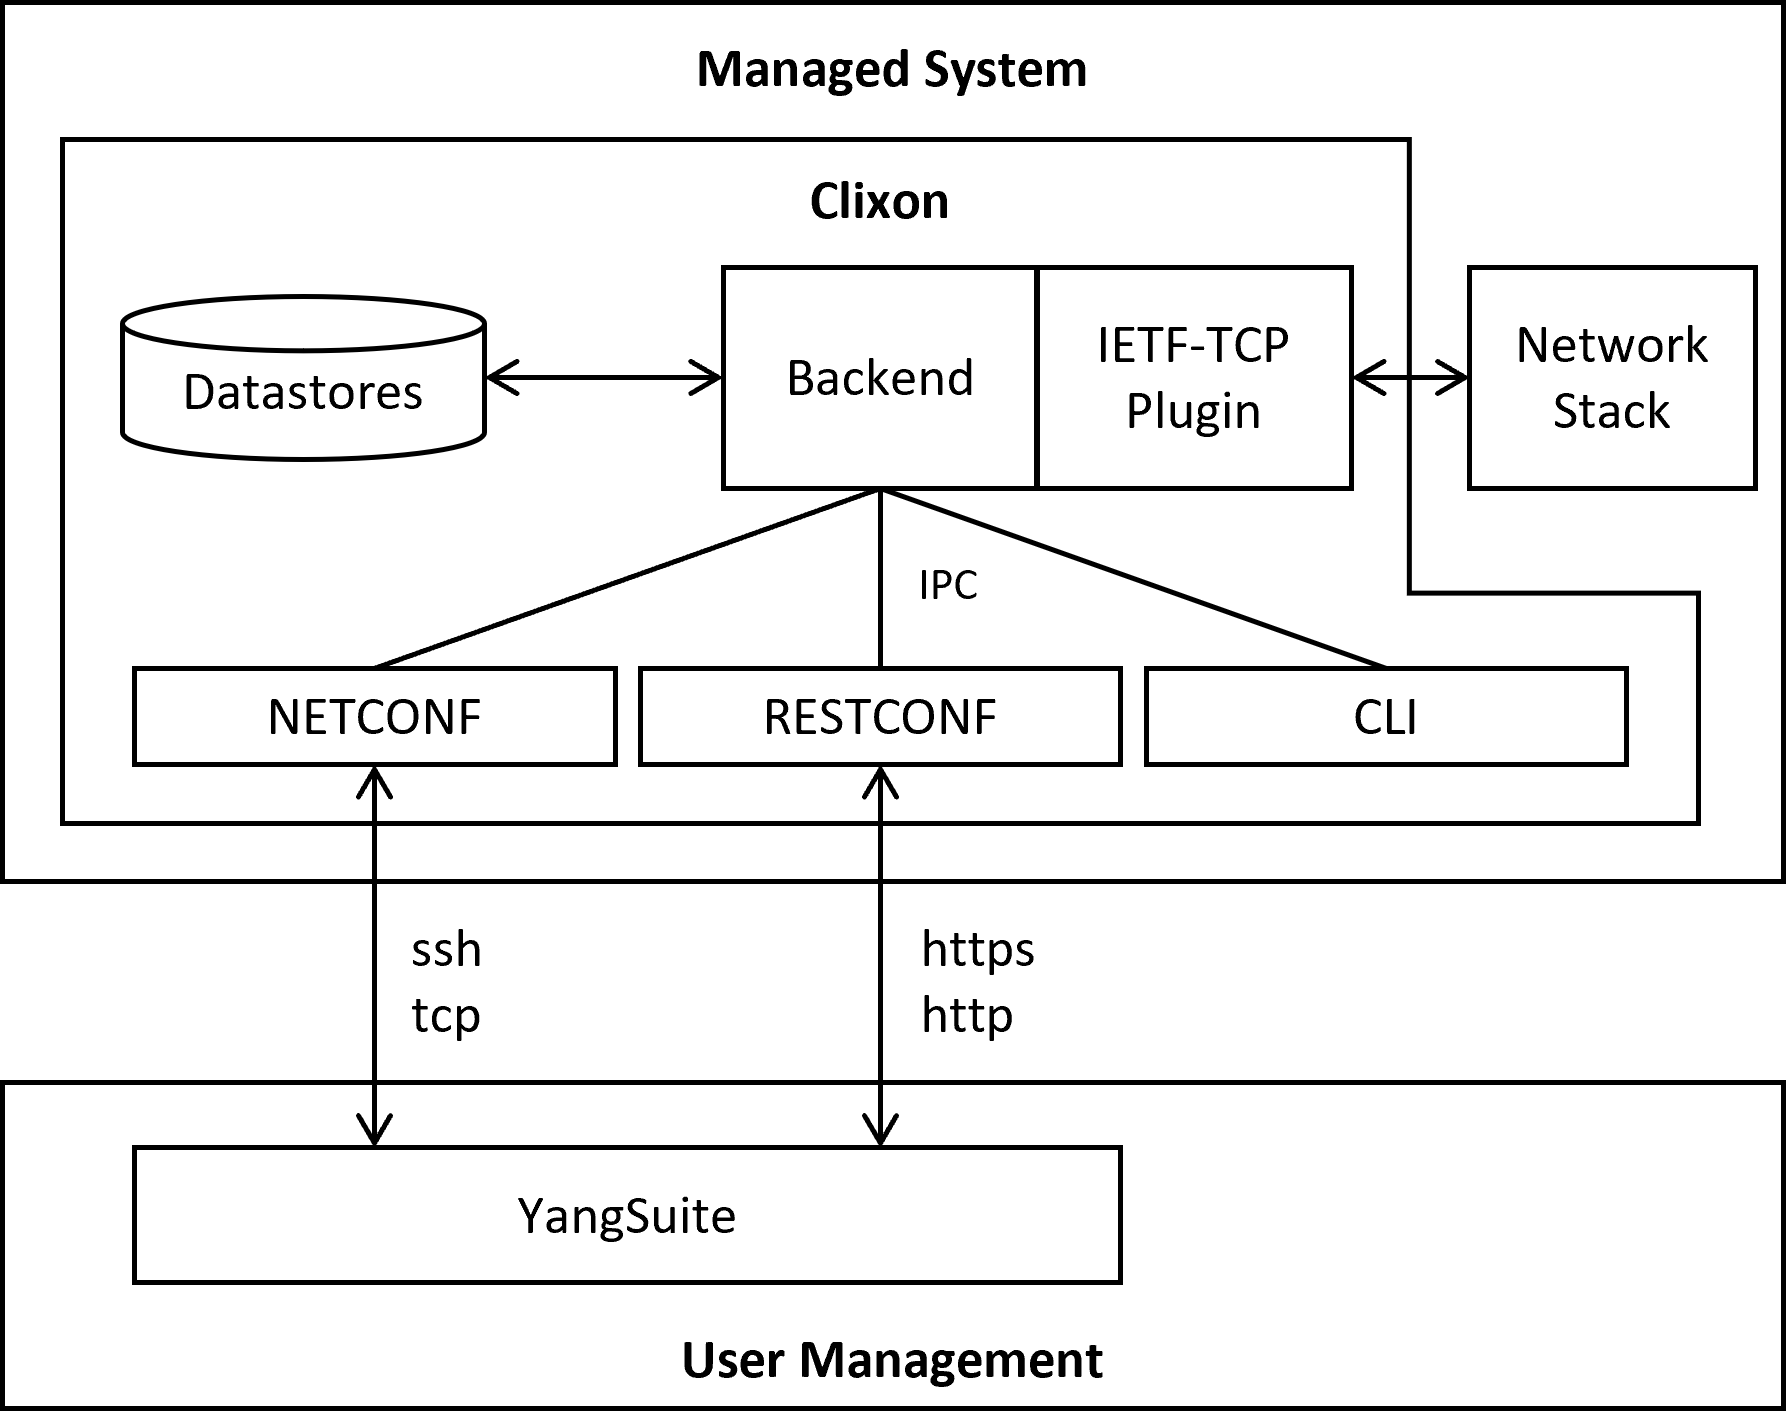
\includegraphics[width=\linewidth]{assets/Prototype/Plugin_Architecture_v.png}
    \caption{Plugin Architecture}
    \label{fig:plugin_architecture}
\end{figure}

Unlike the \textit{Clixon} framework, which is written entirely in \inlinelst{C} and based on the \textit{Autotools toolchain} as the build system, the plugin was developed using \inlinelst{C++} and \textit{CMake} for better development experience.

To obtain the TCP connections and statistics specified in the YANG model from the base system, in this case Ubuntu, the pseudo files \inlinelst{/proc/net/snmp} and \inlinelst{/proc/net/tcp} were read and parsed.

For testing the implementation of the plugin, \textit{YangSuite} was used, which was fairly new at the time of implementation. It provides interfaces like NETCONF and RESTCONF gNMI and and can be operated in a docker container. Fig.~\ref{fig:plugin_architecture} shows how \textit{YangSuite} integrates into the user management layer and into the overall setup.

The Source code for the implemented plugin can be found on GitHub at \url{https://github.com/mager-m/ietf-tcp-research-project}.

%%%%%%%%%%%%%%%%%%
% Portability to QNX
%%%%%%%%%%%%%%%%%%
\subsection{Portability to QNX}
\label{Portability to QNX}

% Why QNX?
QNX is a commercially distributed real time operating system (RTOS) that is used through various industries and serves as the basis is many embedded devices, including network related equipment. Therefore QNX has been chosen as the evaluation platform for the portability analysis. A physical development board, based on the ARMv7 architecture, has been used in the process.

% Technical Prerequisites -> Port Effort 
Since \textit{Clixon}'s goal is to provide a YANG-based configuration manager with support for many platforms, it already runs on a variety of operating systems. To achieve this, \textit{Clixon} relies on different feature flags and the use of \textit{Autotools toolchain} to detect the platform capabilities at configuration time. This not only made it easier to get the framework up and running, but also to adapt any necessary changes as described in the following. 

%& Findings + Challenges
% CLixon
During the deployment of the framework to the new platform a memory corruption appeared while reading the YANG models from the disk. Presumably due to a different memory management it has not been noticed with Ubuntu so far. An appropriate fix was implemented and merged in agreement with the maintainer into the project as pull request.

Another challenge was the lack of support for the multiple privilege functions such as \inlinelst{setresuid} and \inlinelst{getresuid} that are used by \textit{Clixon} to drop privileges after initialization. To overcome this issue, an additional check in \textit{Autotools} along with the feature flag \inlinelst{HAVE\_SETRESUID} was introduced. Thus, if \inlinelst{getresuid} / \inlinelst{setresuid} is not available on the platform, it will be detected during the configuration phase and the relevant code will not be included in the compilation. This change was also merged into the project with a pull request. 

Due to the highly generic code structure, the deployment of the \textit{Clixon} framework to the evaluation platform proceeded without further challenges.

% Plugin
Since QNX does not have the same pseudo files for reading TCP connections and statistics as Ubuntu, modifications to the plugin were necessary. To overcome the non-existent files, the information was obtained by using the \inlinelst{netstat} command and parsing the corresponding output. Otherwise, no major changes were necessary.
    
% Fazit
The deployment of the prototype to the evaluation platform has confirmed the initial assumption and the advertisement of \textit{Clixon}. Due to the generic code base and the use of the \textit{Autotools toolchain} along with many feature flags, the framework proved to be very flexible and easily portable to new UNIX-like environments.

The various challenges faced during the deployment have also highlighted the benefits of open-source software. Besides the possibility to make changes directly to the source code, there is a solid community for emerging questions during the development. Since the changes can be contributed and merged, the framework is constantly evolving and so are the capabilities.

% 
%Since model-based management is also becoming increasingly important in other industries beyond traditional network management, the portability of the implemented software solution was evaluated subsequently.
\section{Related Work}
\label{sec:related-work}

%Building NETCONF-enabled Network Management Systems w/ libnetconf
Krejci (2013)~\cite{libnetconf-krejci} presents the open source library \textit{libnetconf} in his work, which is used by \textit{Netopeer2}. In addition to the various use cases for developing network management applications based on the NETCONF protocol using the presented library, the supported NETCONF capabilities are outlined and guidelines for using the library are given. However, further open-source and commercial YANG-based network software solutions are not compared to the \textit{libnetconf} library in greater detail.

% confD, netopeer,...?

Bajpai and Schönwälder (2014) \cite{netconf-interop-lab} present a NETCONF interoperability lab platform to evaluate NETCONF server and client implementations based on various test-cases. In their work, four different tools are compared, including \textit{YumaPro}, \textit{OpenYuma}, \textit{ConfD} and \textit{libnetconf}.

To our knowledge, there is no other work that analyzes Clixon as a YANG-based network management framework in more detail.


%    Since the standardized and proven technologies such as NETCONF and YANG are increasingly being used in the industry and YANG-based configuration managers are therefore required on the respective devices, it is important to evaluate the tools available on the market. 
\section{Conclusion} 
\label{sec:conclusion}

The prototype has proven that \textit{Clixon} satisfies its claim to be easily adaptable to many platforms and architectures without any substantial changes.
The modular and generic structure of the framework not only allows the mentioned flexibility in terms of operating system or system architecture, but also makes necessary changes much easier, which is an important aspect for development and deployment.

The plugin architecture also proved to be very capable and application-oriented during the development of the prototype due to the existing functionalities of the framework and the accompanying flexibility of the plugins. 

However, the comparison with the two alternatives \textit{Netopeer} and \textit{ConfD} also showed that \textit{Clixon} still has potential for improvement in some areas, such as the partially deviating implementation from the standards.

With regard to the \textit{ietf-tcp} model, there are still a few open topics that can be implemented with upcoming kernel support for the missing authentication features and future releases of the \textit{Clixon} framework.

%%%%%%%%%%%%%%%%%%
% References
%%%%%%%%%%%%%%%%%%

\bibliographystyle{IEEEtran}
\bibliography{IEEEabrv,bib}

\end{document}
